The MiniMax algorithm is a decision rule algorithm for minimizing the
possible loss for a worst case (maximum loss) scenario in a zero sum
game for 2 (or more) players that play in
turns~\cite{Edwards54}.

The algorithm proceeds by building a game tree, where each tree node represents a
game state and the children represent the possible game moves that can
be made by either player 1 or player 2. The
tree levels are built in a way that each player plays in turns and the
first level represents the moves made by player 1.  An
evaluation function \texttt{f(State)} is used to compute the score of
the board for each leaf of the tree. A node is a leaf when it can no longer be
expanded since the state represents a possible end of the game.  Finally, the
algorithm recursively minimizes or maximizes the scores of each node.
To select the best move for player 1, the
algorithm picks the move maximized at the root node.

In LM, the program starts with a root node (with the initial game state)
that is expanded with the available moves at each level. The graph of the
program is dynamic since nodes are created and eventually deleted once they
have nore more facts or no more references to them. The latter happens when the
leaves scores are computed or when a node fully minimizes or maximizes the
children scores. When the program ends, only the root node is have facts in its
database.

The LM code in Fig.~\ref{minimax:check-end} implements
the initial expansion of the tree. The first three rules (lines 1-10) deal
with the cases where no children nodes are created and the last three rules
(12-29) deal with cases where new nodes may be created.
Thes rule in lines 12-25 generate new nodes using the
\texttt{exists} language construct, which creates a new node address
\texttt{B}, where a new \texttt{play} fact is created with the new
board. A \texttt{parent(B,A)} fact is derived to allow node \texttt{B} to
communicate with its parent.

Since our implementation
uses a FIFO ordering for nodes, meaning that when children are expanded, we
first expand each children and then the children of the children. The default
ordering of the system works well enough for most practical purposes. We note
however, that this is not optimal for this program since the complete tree needs
to be expanded before computing the scores at the leaves. This introduces memory
issues since, in the worst case, the space complexity of the program are
$\mathcal{O}(n)$, where $n$ is the number of nodes in the tree.

\begin{figure}[h!]
\scriptsize\begin{Verbatim}[numbers=left,commandchars=\\\{\}]
expand(A, Board, [], 0, P, \underline{Depth})
  -o leaf(A, Board).

expand(A, Board, [], N, P, \underline{Depth}),
N > 0
  -o maximize(A, N, -00, 0).

expand(A, Board, [], N, P, \underline{Depth}),
N > 0, NextPlayer <> RootPlayer
  -o minimize(A, N, +00, 0).

expand(A, Board, [0 | Xs], N, P, Depth),
Depth >= 5
  -o exists B. (\underline{set-static(B)},
       \underline{set-default-priority(B, float(Depth + 1))},
       play(B, Board ++ [P | Xs], next(P), \underline{Depth + 1}),
       expand(A, Board ++ [0], Xs, N + 1, P, \underline{Depth}),
       parent(B, A)).

expand(A, Board, [0 | Xs], N, P, Depth),
Depth < 5
  -o exists B. (\underline{set-default-priority(B, float(Depth + 1))},
       play(B, Board ++ [P | Xs], next(P), \underline{Depth + 1}),
       expand(A, Board ++ [0], Xs, N + 1, P, \underline{Depth}),
       parent(B, A)).

expand(A, Board, [C | Xs], N, P, \underline{Depth})
C <> 0
  -o expand(A, Board ++ [C], Xs, N, P, \underline{Depth}).
\end{Verbatim}
\caption{MiniMax: checking if the game has ended and expanding the tree}
\label{minimax:check-end}
\end{figure}
\normalsize

With coordination, we set the priority nodes to be the same as the
depth so that the tree is expanded in a depth-first fashion (lines 15 and 22).
The memory complexity of the program then becomes $\mathcal{O}(d t)$, where $d$
is the depth of the tree and $t$ is the number of threads. In
Fig.~\ref{fig:minimax}, we have two threads (squares) and the first one has
expanded the tree on the left side. When a second thread comes up, it steals the
first unexpanded node and expands the tree from that position. Since threads
prioritize deeper nodes, the scores of the first leaves are immediatelly
computed and then sent to the parent node. At this point, the leaves are deleted
and reused for other nodes in the tree, resulting in minimal memory usage.

\begin{figure}[h!]
   \begin{center}
      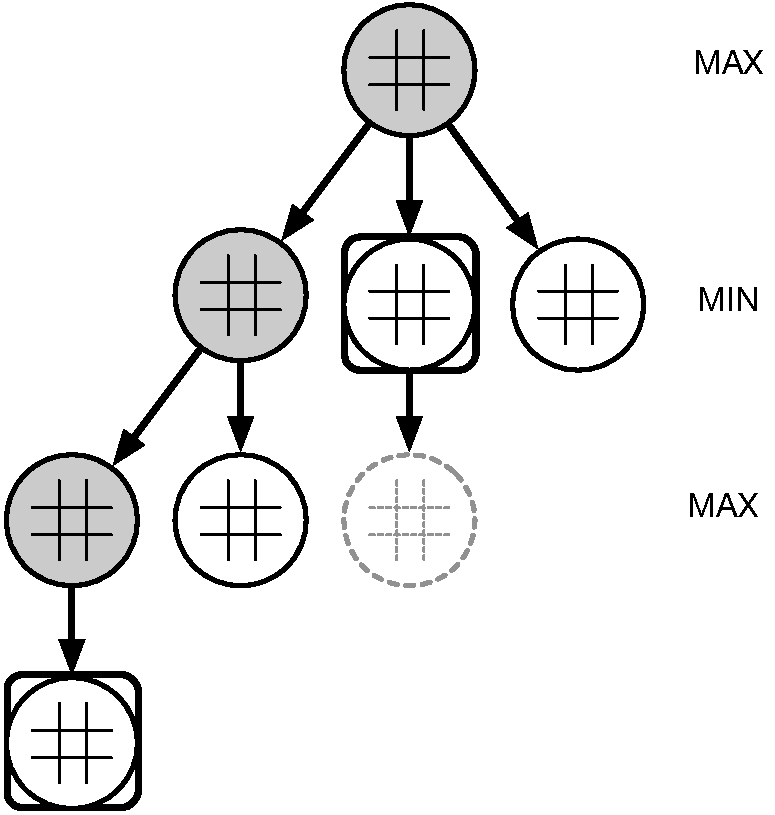
\includegraphics[width=4.5cm]{figures/minimax_tree}
   \end{center}
   \caption{Expanding the MiniMax tree using coordination. By prioritizing
      deeper nodes, threads are forced to expand the tree using a depth-first
      approach, which is superior since there is no need to expand the whole
      tree before computing the node scores.}
   \label{fig:minimax}
\end{figure}

We also take advantage of memory locality by using \texttt{set-static} (line
14), so that nodes after a certain level are not stolen by other threads. While
this is not critical for performance in shared memory systems where node
stealing is fairly efficient, we expect that such coordination to be critical in
distributed systems.

\begin{figure}[h!]
   \begin{center}
      \subfloat[]{ \begin{tabular}[b]{ | c | c | c |}
         \hline                       
         \textbf{\# T} & \textbf{R} & \textbf{C} \\ \hline \hline
         1 & 11.80GB & 0.50MB \\ \hline
         2 & 12.19GB & 1.45MB \\ \hline
         4 & 13.82GB & 2.35MB \\ \hline
         8 & 14.87GB & 4.36MB \\ \hline
         16 & 13.79GB & 8.1MB \\ \hline
         \end{tabular}
         \normalsize
      }
      \subfloat[]{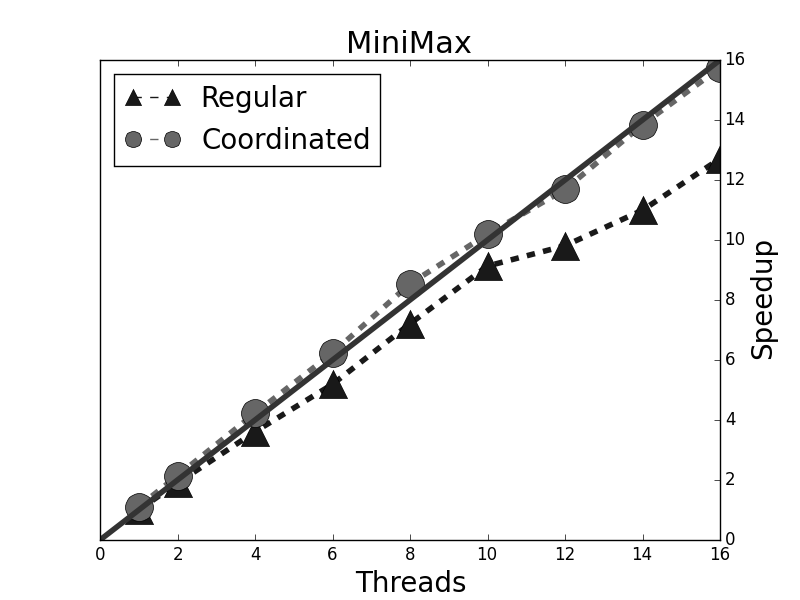
\includegraphics[width=5cm]{results/min-max-tictactoe.png}}
   \end{center}
   \caption{Memory usage and scalability of the regular and coordinated versions
      of MiniMax.}
   \label{results:memory_minmax}
\end{figure}

